\documentclass[tikz,border=1.35mm]{standalone}
\usetikzlibrary{arrows.meta}

\definecolor{externalface}{HTML}{8FB9E8}
\definecolor{internalface}{HTML}{F4B46A}
\definecolor{splitred}{HTML}{AF2525}
\definecolor{centroidgreen}{HTML}{0E8814}

% Experimental colored isotropic-refinement prism figure.
% The triangular faces lie in the z=0 and z=1 planes; the extrusion is along z.
% Blue faces are exterior faces; amber faces are internal faces introduced by refinement.
\begin{document}
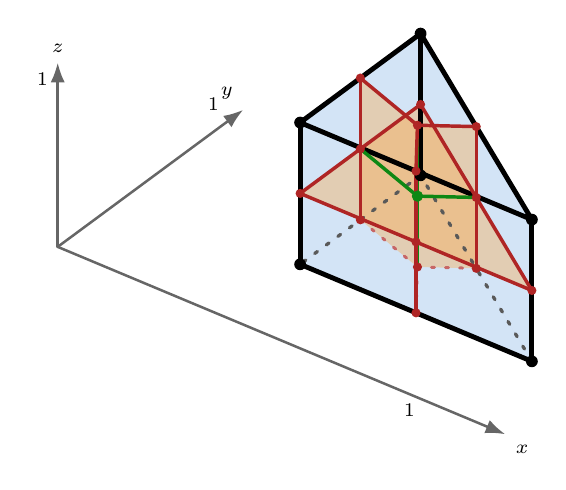
\begin{tikzpicture}[
  x={(20.3mm,-8.5mm)},
  y={(15.3mm,11.3mm)},
  z={(0mm,18mm)},
  line join=round,
  line cap=round,
  outer/.style={draw=black,line width=0.62mm},
  split/.style={draw=splitred,line width=0.44mm},
  centroidedge/.style={draw=centroidgreen,line width=0.44mm},
  hidden/.style={draw=black!65,line width=0.42mm,loosely dotted},
  hiddensplit/.style={draw=splitred!70,line width=0.38mm,loosely dotted},
  exterior/.style={fill=externalface,fill opacity=0.22,draw=none},
  interior/.style={fill=internalface,fill opacity=0.48,draw=none},
  axis/.style={draw=black!60,line width=0.32mm,-{Latex[length=2.5mm,width=1.8mm]}}
]
  % Right-triangular prism vertices, stretched in x for visual clarity.
  \coordinate (A) at (0,0,0);
  \coordinate (B) at (1.45,0,0);
  \coordinate (C) at (0,1,0);
  \coordinate (D) at (0,0,1);
  \coordinate (E) at (1.45,0,1);
  \coordinate (F) at (0,1,1);

  % Edge midpoints.
  \coordinate (mAB) at (0.725,0,0);
  \coordinate (mBC) at (0.725,0.5,0);
  \coordinate (mCA) at (0,0.5,0);
  \coordinate (mDE) at (0.725,0,1);
  \coordinate (mEF) at (0.725,0.5,1);
  \coordinate (mFD) at (0,0.5,1);
  \coordinate (mAD) at (0,0,0.5);
  \coordinate (mBE) at (1.45,0,0.5);
  \coordinate (mCF) at (0,1,0.5);

  % Face centroids and element centroid.
  \coordinate (fABC) at (0.483,0.333,0);
  \coordinate (fDEF) at (0.483,0.333,1);
  \coordinate (fABED) at (0.725,0,0.5);
  \coordinate (fADFC) at (0,0.5,0.5);
  \coordinate (fBCEF) at (0.725,0.5,0.5);
  \coordinate (center) at (0.483,0.333,0.5);

  % Offset coordinate axes; ticks mark one unit in each direction.
  \coordinate (Oaxis) at (-1.20,-0.42,-0.18);
  \draw[axis] (Oaxis) -- (1.60,-0.42,-0.18) node[below right,font=\scriptsize] {$x$};
  \draw[axis] (Oaxis) -- (-1.20,1.12,-0.18) node[above left,font=\scriptsize] {$y$};
  \draw[axis] (Oaxis) -- (-1.20,-0.42,1.12) node[above,font=\scriptsize] {$z$};
  \node[font=\scriptsize,below] at (1.00,-0.42,-0.18) {$1$};
  \node[font=\scriptsize,above left] at (-1.20,1.00,-0.18) {$1$};
  \node[font=\scriptsize,left] at (-1.20,-0.42,1.00) {$1$};

  % Exterior faces remain blue so the original cell boundary stays legible.
  \path[exterior] (A) -- (B) -- (C) -- cycle;
  \path[exterior] (D) -- (E) -- (F) -- cycle;
  \path[exterior] (A) -- (B) -- (E) -- (D) -- cycle;
  \path[exterior] (B) -- (C) -- (F) -- (E) -- cycle;
  \path[exterior] (C) -- (A) -- (D) -- (F) -- cycle;

  % Internal refinement faces, one quadrilateral for each original edge.
  \path[interior] (mAB) -- (fABC) -- (center) -- (fABED) -- cycle;
  \path[interior] (mBC) -- (fABC) -- (center) -- (fBCEF) -- cycle;
  \path[interior] (mCA) -- (fABC) -- (center) -- (fADFC) -- cycle;
  \path[interior] (mDE) -- (fDEF) -- (center) -- (fABED) -- cycle;
  \path[interior] (mEF) -- (fDEF) -- (center) -- (fBCEF) -- cycle;
  \path[interior] (mFD) -- (fDEF) -- (center) -- (fADFC) -- cycle;
  \path[interior] (mAD) -- (fABED) -- (center) -- (fADFC) -- cycle;
  \path[interior] (mBE) -- (fABED) -- (center) -- (fBCEF) -- cycle;
  \path[interior] (mCF) -- (fADFC) -- (center) -- (fBCEF) -- cycle;

  % Hidden-line convention: only the back edges of the lower face are dotted.
  \draw[hidden] (B) -- (mBC) -- (C) -- (mCA) -- (A);

  % Visible exterior split topology.
  \draw[outer] (A) -- (mAB) -- (B);
  \draw[outer] (D) -- (mDE) -- (E) -- (mEF) -- (F) -- (mFD) -- cycle;
  \draw[outer] (A) -- (mAD) -- (D);
  \draw[outer] (B) -- (mBE) -- (E);
  \draw[outer] (C) -- (mCF) -- (F);

  % New face-centroid to element-centroid edges.
  \draw[centroidedge] (center) -- (fABC);
  \draw[centroidedge] (center) -- (fDEF);
  \draw[centroidedge] (center) -- (fABED);
  \draw[centroidedge] (center) -- (fADFC);
  \draw[centroidedge] (center) -- (fBCEF);

  % Face-centroid connections on exterior faces.
  \draw[hiddensplit] (fABC) -- (mAB);
  \draw[hiddensplit] (fABC) -- (mBC);
  \draw[hiddensplit] (fABC) -- (mCA);
  \draw[split] (fDEF) -- (mDE);
  \draw[split] (fDEF) -- (mEF);
  \draw[split] (fDEF) -- (mFD);
  \draw[split] (fABED) -- (mAB);
  \draw[split] (fABED) -- (mBE);
  \draw[split] (fABED) -- (mDE);
  \draw[split] (fABED) -- (mAD);
  \draw[split] (fADFC) -- (mAD);
  \draw[split] (fADFC) -- (mFD);
  \draw[split] (fADFC) -- (mCF);
  \draw[split] (fADFC) -- (mCA);
  \draw[split] (fBCEF) -- (mBE);
  \draw[split] (fBCEF) -- (mBC);
  \draw[split] (fBCEF) -- (mCF);
  \draw[split] (fBCEF) -- (mEF);

  % Original vertices are black; edge and face refinement nodes are red.
  \foreach \p in {A,B,C,D,E,F} {
    \fill[black] (\p) circle[radius=0.75mm];
  }
  \foreach \p in {mAB,mBC,mCA,mDE,mEF,mFD,mAD,mBE,mCF,
                  fABC,fDEF,fABED,fADFC,fBCEF} {
    \fill[splitred] (\p) circle[radius=0.58mm];
  }
  \fill[centroidgreen] (center) circle[radius=0.72mm];
\end{tikzpicture}
\end{document}
